\section{Additive Nethoden}\label{sec:add}


\subsection{Verringerung der für Berechnungen nötige Zeit}\label{sec:fp16}
\todo[inline]{Überarbeiten, fertigschreiben; 3 Stunden}



Die Zeit, die ein Convolutional Layer braucht um berechnet zu werden hängt ab von:
\begin{itemize}
 \item dem verwendeten Zahlenformat
 \item der Filtergr\"osse
 \item der Bildgr\"osse
 \item dem verwendetem Stride und Padding
\end{itemize}



Beim Verändern der Filter- oder der Bildgr\"osse, um Trainingszeit zu sparen, ver\"andert sich auch die Erkennungsleistung \todo{cite}. Dies ist beim Verändern des verwendeten Zahlenformats nicht umbedingt gegeben. Standardformat ist eine 32 Bit Gleitkommazahl. Die einfachste Methode hier Trainingszeit zu sparen ist das Halbieren der Bitanzahl auf 16 Bit. Eine weitere Methode ist das Benutzen von 16 Bit Dynamischen Festkommazahlen.
Die beiden alternativen Methoden haben unterschiedliche Anforderungen an die Ausführungsplattform. Diese Anforderungen und die Besonderheiten der beiden Verfahren werden in den folgenden zwei Unterkapiteln näher beleuchtet.


\paragraph{Berechnung mit 16 Bit Gleitkomma}
\cite{ieee}
Die 16 Bit Gleitkommazahl unterscheidet sich nicht nur in der Länge von der 32 Bit Zahl sondern aus der unterschiedlichen Länge erwachsen Unterschiede in den darstellbaren Zahlen. In Tabelle \ref{tab:numbers} sind diese Unterschiede dargestellt. 

\begin{table}[H]
\captionof{table}{Darstellbare Zahlen von 16 und 32 Bit}
\label{tab:numbers}
\begin{tabular}{|c|c|c|}
\hline                                       & 16 Bit                             & 32 Bit              \\ \hline
kleinste darstellbare positive Zahl    & $0.61  \cdot 10^{-4}$              & $1.1755 \cdot 10^{-38}$ \\ \hline
grösste darstellbare positive Ganzzahl & $65504$                            & $ 3.403 \cdot 10^{38}$  \\ \hline
minimal subnormale Zahl                & $2^{-24} \approxeq 5.96 \cdot 10^{-8}$ & $ 2^{-149}$         \\ \hline
\end{tabular}
\end{table}

Subnormale Zalen ergeben sich, wenn der Exponent 0 ist und \todo[inline]{subnormale Zahlen}

Durch diese Unterschiede im Umfang der darstellbaren Zahlen ergibt sich ein direkter Unterschied im Training eines CNNs. Durch den Wechsel auf 16 Bit ist ein bestimmter Teil der Gradienten gleich Null. 

Diese Nachteile von 16 Bit Gleitkommazahlen können durch drei Techniken abgemeildert oder sogar komplett aufgehoben werden:
\begin{itemize}
 \item 32 Bit Mastergewichte und Updates
 \item Sklaierung der Loss-Funktion
 \item Arithmetische Präzision 
\end{itemize}

Beim Trainieren von neuronalen Netzwerken mit 16 Bit Gleitkommazahlen werden die Gewichte, Aktivierungen und Gradienten im 16 Bit Format gespeichert. Die Speicherung der Gewichte als 32 Bit Mastergewichte hat zwei mögliche Erklärungen, die aber nicht immer zutreffen müssen. 

Um nach einem Forward Druchlauf des Netzes die Gewichte abzudaten wird ein Gradientenabstiegsverfahren benutzt. Hierbei werden die Gradienten der Gewichte berechnet. Um für die Funktion, die das CNN approximiert einen besseren Approximationserfolg zu erlangen wird dann dieser Gradient mit der Lernrate multipliziert. Wird dieses Produkt in 16 Bit abgespeichert, so ist in viele Fällen das Produkt der beiden Zahlen gleich Null. Dies liegt an der Taqtsache, dass wie in Tabelle \todo{ref} zu sehen ist die kleinste darstellbare Zahl in 16 Bit wesentlich grösser ist als in 32 Bit.


Der zweite Grund wieso man Mastergewichte brauchen könnte ist die Tatsache, dass bei grossen Gewichten die Länge der Mantisse nicht ausreicht, um sowohl das Gewicht als auch das zu  addierende Update zu speichern.

Aus den beiden Gründen wird das in Abbildung \ref{abb:mixed} gezeigte Schema zum Trainieren einer Schicht mit gemischt präzisen Gleitkommazahlen benutzt.

\begin{figure}[h]
 \centering
 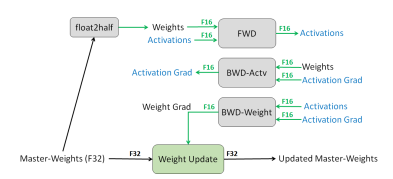
\includegraphics[width=0.8 \textwidth]{KapitelPartA/images/mixed.png}
 % mixed.png: 393x179 px, 72dpi, 13.86x6.31 cm, bb=0 0 393 179
 \label{abb:mixed}
\end{figure}



